\documentclass[conference]{IEEEtran}
\usepackage{graphicx}
\usepackage{tikz}
\usepackage{float}
\usepackage{pgfplots}
\pgfplotsset{compat=1.18}
\usepackage{hyperref}
\usepackage{amsmath,amssymb}
\usepackage{algorithm}        
\usepackage[noend]{algpseudocode} 
\usepackage{listings}
\usepackage{adjustbox}
\usetikzlibrary{shapes.geometric, arrows.meta, positioning, fit, shadows, patterns}
\usepackage{placeins}
\usepackage{stfloats}
\usepackage[
  protrusion=true,
  activate={true,nocompatibility},
  final,
  tracking=true,
  kerning=true,
  spacing=true,
  factor=1100]{microtype}
\SetTracking{encoding={*}, shape=sc}{40}
\usepackage{inconsolata}            
\usepackage{xcolor}               
\lstdefinestyle{rgcode}{
  language=C,
  basicstyle=\scriptsize\ttfamily,  
  numbers=left, numberstyle=\tiny,
  numbersep=6pt, xleftmargin=2em,
  frame=lines, rulecolor=\color{black},
  breaklines=true, breakindent=0pt,
  showstringspaces=false,
  captionpos=b
}
\lstset{
    basicstyle=\small\ttfamily,
    breaklines=true,
    frame=single,
    numbers=none,
    showstringspaces=false,
    morekeywords={uint\_32t, struct, int64\_t},
    keywordstyle=\color{blue},
    stringstyle=\color{red},
    commentstyle=\color{green!60!black},
    columns=flexible,
    keepspaces=true,
}
\title{Remember Glaze: A High Throughput Persistence Mechanism}
\author{Paul Louis Robert Quesnot}
\begin{document}

\maketitle

\begin{abstract}
   Modern ledgers and databases still pair write-ahead logging with periodic snapshots, incurring long pauses, while chunk-based Glaze breaks down on bulk updates. Remember Glaze removes both limits. It slices state into fixed-size chunks stored in a circular ring log; each batch appends only the modified chunk plus its transaction list, giving constant-time commits and a strictly bounded disk footprint. Crash recovery touches at most one snapshot per chunk and replays only the missing batches. On a 100 M-account benchmark this cuts median per-batch latency by 40–70 \% against the previous standard and rebuilds the full state in a couple of minutes. \textit{Remember Glaze} is therefore a practical drop-in for high-throughput systems that demand predictable latency and rapid restart.
\end{abstract}

\section{Introduction}
\subsection{Motivation}

Modern high-throughput systems (blockchains, large databases) must apply millions of updates per second and still recover fully after a crash.  The dominant technique—write-ahead logging plus periodic full snapshots—meets crash-consistency requirements but introduces “latency cliffs”: long pauses whenever a gigabyte-scale snapshot is flushed to disk.  With state sizes already in the multi-terabyte range (e.g., Ethereum archive nodes) and projected to reach billions of accounts, even small per-batch slowdowns accumulate into hours of lost throughput each day. Yet no existing method simultaneously offers :

\begin{enumerate}
    \item \emph{Constant-time} commits independent of state size,
    \item Graceful handling of arbitrarily large, non-interdependent writes, and
    \item A deterministically bounded on-disk footprint.
\end{enumerate}

\textit{Remember Glaze} is motivated by this gap.  The goal of this report is to design and evaluate a persistence layer that preserves the simplicity and cache efficiency of in-memory processing while offering disk durability with \emph{zero snapshot spikes}, predictable resource usage, first-class support both for bulk state transformations as well programs leveraging spatial locality.  Achieving these properties simultaneously would remove one of the main performance bottlenecks in next-generation database and blockchain infrastructures and establish clear guidelines for
future system architects.

\subsection{Contributions}

This project acts as an addition to the arena of high-throughput, crash-resistant data stores by introducing \textit{Remember Glaze}, a persistence mechanism specifically designed to address existing limitations in state management systems.

Its main contributions can be summarized in the following points: 
\begin{itemize}
\item \textbf{Function-centric batch commits:} Remember Glaze ensures that the complexity of batch transactions is solely determined by the applied state transformation functions, rather than by persistence mechanics.
\item \textbf{State-size-independent performance:} Execution speed remains constant regardless of the state’s size, guaranteeing predictable and efficient processing times.
\item \textbf{Deterministically bounded on-disk storage:} Our architecture precisely defines disk space requirements in advance, effectively preventing storage-related issues that arise from continuously expanding log files.
\item \textbf{Decoupled transaction execution and persistence:} A clear architectural distinction between the execution of transactions and  state persistence simplifies the system, improving maintainability and scalability.
\item \textbf{Highly tunable execution:} Our model enables us to tune several parameters to optimize for different use cases. 
\end{itemize}
In this report, we synthesize practical applications of \textit{Remember Glaze}, thereby giving empirically supported insights in selecting optimal parameters to balance throughput, latency, and recovery objectives effectively.
\section{Background}

Persistence and recovery strategies in modern data-intensive applications primarily follow two major paradigms: write-ahead logging combined with periodic snapshotting, and log-structured or incremental checkpointing approaches. This section details these methodologies, discusses their advantages and limitations, and introduces the \textit{Glaze} and \textit{WAL-snapshot} baselines to provide context for our proposed \textit{Remember Glaze} solution.

\subsection{Write-Ahead Logging (WAL) with Snapshots}

This paradigm underpins numerous transactional database systems, such as PostgreSQL \cite{postgresql_docs} and Cassandra \cite{lakshman2010cassandra}. WAL ensures durability by logging every transaction to persistent storage before applying changes in memory. Periodically, these systems generate a complete snapshot of the current in-memory state, persisting it to disk and subsequently truncating the log. Recovery then involves loading the latest snapshot and replaying logged transactions to reconstruct the most recent consistent state \cite{mohan1992aries}.

While WAL-snapshot methods offer robust crash consistency and support fine-grained locking and rollbacks \cite{mohan1992aries}, their significant drawback lies in periodic snapshots. Snapshotting incurs substantial I/O overhead proportional to the total state size, resulting in latency spikes or "latency cliffs". These pauses become critical performance bottlenecks, particularly in high-throughput, large-scale systems managing terabytes of state \cite{kalantar1998oracle}.

\subsection{Log-Structured and LSM-Tree Architectures}

Log-structured storage systems mitigate random write overhead by sequentially appending updates to a log. The seminal \textit{Log-Structured File System (LFS)} \cite{rosenblum1992lfs} pioneered this concept, enhancing write performance by reducing random disk seeks. Extending this concept, \textit{Log-Structured Merge-Trees (LSM-Trees)} structure data into sorted levels and periodically compact these levels to remove outdated entries \cite{o1996lsm}. Systems like LevelDB and RocksDB exemplify the LSM paradigm, delivering high sustained write throughput.

However, these systems experience periodic background compaction stalls, where compaction operations consume significant CPU and I/O resources. As data scales, compaction overhead can degrade overall system performance \cite{o1996lsm,ongaro2020efficient}.

\subsection{Incremental Checkpointing and Chunk-Based Approaches}

Incremental checkpointing schemes, such as Apache Flink’s incremental checkpoints \cite{carbone2015flink} and Oracle’s incremental buffer-pool checkpoints \cite{kalantar1998oracle}, address the drawbacks of full snapshots and background compactions by only persisting modified state portions since the last checkpoint. Such methods considerably reduce I/O and pause durations but still occasionally require full snapshots to ensure comprehensive recoverability.

The original \textit{Glaze} design further advances incremental checkpointing by logically dividing the entire state into equally sized chunks, each stored in a circular buffer on disk. After processing each batch, only the chunk modified in memory and its associated write-set are persisted. This strategy ensures constant-size writes per batch, bounding storage overhead and smoothing out latency. During recovery, \textit{Glaze} loads the most recent snapshot of each chunk and replays corresponding logs to reconstruct the state incrementally.

Despite improvements, \textit{Glaze} encounters performance issues when processing large non-interdependent writes, such as extensive \texttt{memset}-type operations. These writes trigger full chunk rewrites and exponentially growing log files, creating substantial overhead for each affected batch.

\subsection{Summary of Baseline Trade-Offs}

\begin{itemize}
\item \textbf{WAL-Snapshot:} Ensures strong consistency and durability \cite{mohan1992aries}, but periodic full snapshots cause latency spikes proportional to state size \cite{kalantar1998oracle}.
\item \cite{ono1996lsm} Achieves high sustained write throughput through sequential log appends \cite{rosenblum1992lfs}, but incurs pronounced compaction-related stalls at scale \cite{ono1996lsm}.
\item \textbf{Incremental / Chunk-Based (Glaze):} Offers bounded storage overhead and constant-size writes per batch, yet large non-interdependent writes cause considerable per-chunk rewrite overhead.
\end{itemize}

These limitations directly motivate \textit{Remember Glaze}, an enhanced chunk-based persistence solution designed explicitly to handle large bulk updates efficiently, guarantee constant-time batch commits independent of state size, and maintain a deterministically bounded disk footprint. The subsequent sections elaborate on how \textit{Remember Glaze} addresses these specific shortcomings.
\section{Implementation and Design}

\subsection{Design}
\paragraph{General Structure}
The design of \textit{Remember Glaze} emphasizes efficiency and robustness in state persistence by utilizing a hybrid in-memory and on-disk architecture. The overall application state, represented as an array of account balances, is primarily kept in main memory to leverage fast access speeds. For durability, the system employs a circular ring buffer stored on disk, termed the \textit{checkpoint ring log}. This ring log structure comprises snapshot slots for storing discrete state chunks and associated transaction slots, which record the batch of transactions that got executed at the same epoch as the state chunk was persisted.

\paragraph{Separation of Transaction Processing and State Commitment}
A core design decision involves separating transaction execution from state persistence. The execution engine focuses purely on in-memory operations, optimized for cache locality and parallel execution. Meanwhile, the durability layer asynchronously serializes only the modified state chunk and its corresponding transaction log to disk after each batch execution, significantly reducing the overhead of persistent storage operations.

\paragraph{Commitment }
When a new batch b of transactions arrives, Remember Glaze first applies each transaction in memory to only the affected chunk c, where c = b $\bmod$ N, N the total number of chunks in the ring. Because each chunk holds a fixed subset of account state, all writes for transactions touching those accounts stay confined to that one chunk. Once the in‐memory updates complete, the system commits the changes by writing exactly one new snapshot of chunk c back into the circular ring buffer on disk . Underneath that chunk snapshot, there is a parallel “Batch b” slot in the transaction log area holding the metadata and transaction payloads for batch b. Together, these two pieces occupy exactly one fixed‐size slot in the checkpoint ring. On the next batch, the ring pointer advances to (b+1) $\bmod$ N, so when you circle around after N batches, the oldest chunk and log entries are automatically overwritten. In this way, each batch commit consists of one copy of a single chunk plus one write of the batch log; no matter how large the entire state grows, every commit always writes exactly the same amount of data. This guarantees bounded disk usage and a constant, predictable persistence overhead per batch, eliminating any need for full‐state snapshots or large, variable‐length writes during steady‐state processing.

\begin{figure*}[!t]
\centering
\includegraphics[width=\textwidth]{Images/Commitment.pdf}
\caption{Transaction processing in Remember Glaze.
Incoming batches are applied in memory chunk by chunk; only the modified chunk is written
into the circular ring buffer on disk. This guarantees that each batch’s persistence
cost remains constant (independent of total state size), bounding I/O overhead.}
\label{fig:transaction_processing_fullwidth}
\end{figure*}

\noindent
Figure \ref{fig:transaction_processing_fullwidth} shows how each batch “b”
is applied to memory and then flushed to disk \emph{only} at the single chunk index
c = b $\bmod$ N. As a result, while memory operations touch only chunk c
in RAM, persistence happens via a fixed‐size write into the circular buffer,
eliminating any full‐state snapshots or large writes during steady‐state execution.

\paragraph{Recovery }
Upon startup or after a crash, the \textit{Remember Glaze} system restores its in-memory state by reading and replaying the checkpoint ring log. The recovery procedure proceeds in three main phases: (1) validate and parse the checkpoint header, (2) load the most recent chunked snapshot for each state region, and (3) replay any missing transactions to advance each chunk from its snapshot batch to the overall latest batch. By organizing chunks in a fixed-size circular buffer, the algorithm bounds both disk usage and recovery work. The pseudo-code for the algorithm is the following: 
\begin{algorithm}[H]
\scriptsize
\caption{Recovery Algorithm (Pseudocode)}
\begin{algorithmic}[1]
\Function{RecoverStateFromLog}{log\_fd}
    \State header \(\leftarrow\) \Call{ReadCheckpointHeader}{log\_fd}
    \If{header invalid or parameters mismatch}
        \State \Return \(\text{Error: cannot recover}\)
    \EndIf
    \State \(N \leftarrow \text{NUM\_STATE\_CHUNKS}\)
    \State \(\text{batchNum}[0..N-1] \leftarrow -1\)
    \State \(\text{maxBatch} \leftarrow -1\)
    \State \(\text{latestIdx} \leftarrow -1\)
    \For{\(k = 0\) \textbf{to} \(N-1\)}
        \State snapSlot \(\leftarrow\) \Call{ReadChunkSlot}{log\_fd, offset\_for\_chunk(k)}
        \If{(\(snapSlot.chunk\_idx == k\)) \textbf{and} 
        
        (\(snapSlot.batch\_num > \text{batchNum}[k]\))}
            \State \(\text{batchNum}[k] \leftarrow snapSlot.batch\_num\)
            \If{\(\text{batchNum}[k] > \text{maxBatch}\)}
                \State \(\text{maxBatch} \leftarrow \text{batchNum}[k]\)
                \State \(\text{latestIdx} \leftarrow k\)
            \EndIf
        \EndIf
    \EndFor
    \If{\(\text{latestIdx} < 0\)}
        \State \Return \(\text{Error: no valid snapshot found}\)
    \EndIf
    \State Initialize \(\text{stateArray} \leftarrow \mathbf{0}\)
    \For{\(k = 0\) \textbf{to} \(N-1\)}
        \If{\(\text{batchNum}[k] \ge 0\)}
            \State \(\text{chunkData} \leftarrow\) \Call{ReadSnapshotData}{log\_fd, k}
            \State \(\text{CopyIntoState}(\text{stateArray}, k, \text{chunkData})\)
        \EndIf
    \EndFor
    \State \(\text{lastRecoveredBatch} \leftarrow \text{maxBatch}\)
    \For{\(\Delta = 1\) \textbf{to} \(N-1\)}
        \State \(k \leftarrow (\,\text{latestIdx} - \Delta\,) \bmod N\)
        \For{batch = \(\text{batchNum}[k] + 1\) \textbf{to} \(\text{maxBatch}\)}
            \State slotIdx \(\leftarrow\) \(batch \bmod N\)
            \State txSlot \(\leftarrow\) \Call{ReadBatchSlot}{log\_fd, slotIdx}
            \For{each transaction \(\tau\) in \(\text{txSlot.transactions}\)}
                \If{\(\tau\) affects chunk \(k\)}
                    \State \Call{ApplyTransaction}{stateArray, \(\tau\)}
                \EndIf
            \EndFor
        \EndFor
    \EndFor
    \State \Return \(\text{stateArray},\,\text{lastRecoveredBatch}\)
\EndFunction
\end{algorithmic}
\end{algorithm}

\paragraph{Complexity Analysis}
This design ensures that recovery work is bounded by $O(NS + N^2B)$, where $N$ is the number of chunks (for loading snapshots), $S$ is the size of each account, and $NS$ is therefore the total size of the chunks in bytes in the chunkSlots. $B$ is the batch size in number of transactions. Phase 2 reads and copies one chunk snapshot for each of the N chunks, so the cost is $O(NS)$. Phase 3 replays at most $N$ batches for each chunk; each batch contains at most $B$ transactions, giving $O(N × N × B)=O(N^{2}B)$.
Header parsing and the initial metadata scan add only O(N) and do not change the leading term. Hence the worst-case recovery work is $O(NS + N^{2}B)$. In typical random-access workloads the replay term drops to $O(NB)$ because only roughly $1/N$ of the transactions affect a given chunk.

By never writing a full state dump and instead relying on fixed‐size chunk slots plus transaction slots, \textit{Remember Glaze} guarantees a predictable on‐disk footprint and a deterministic recovery path.

Critical design parameters, such as chunk size, batch size, and the number of state chunks, are configurable at compile-time. These parameters represent important trade-offs between steady-state processing speed and recovery complexity, allowing the system to be tailored to specific operational requirements.
\FloatBarrier
\begin{figure*}[!t]
  \centering
  \includegraphics[width=\textwidth]{Images/Recovery.pdf}
  \caption{Recovery in Remember Glaze. 
    After a crash, all chunk slots on disk are first loaded into memory in reverse 
    circular order (starting from the most recent chunk index $c$). Then, every 
    transaction up to batch $b$ in each chunk slot is conditionally applied to 
    reconstruct the full state. Ultimately, only missing transactions (per chunk) 
    are replayed, guaranteeing deterministic and bounded recovery work.}
  \label{fig:recovery_fullwidth}
\end{figure*}
\noindent
Figure \ref{fig:recovery_fullwidth} illustrates the recovery path. At startup, 
Remember Glaze scans the on‐disk ring buffer to find the latest valid chunk index $c$ 
(i.e., max batch number). It then copies each chunk’s snapshot into memory—loading 
“chunk $c+1$” first (wrapping around), “chunk $c+2$”, and so on—so that each chunk 
ends up at its most recent snapshot. Finally, it conditionally replays any 
transactions whose batch numbers exceed that chunk’s snapshot batch, guaranteeing 
that the in-memory state is fully up to date with batch $b$ without ever doing a 
full-state read or log replay.
\FloatBarrier
\subsection{Implementation}

The implementation of \textit{Remember Glaze} is designed for simplicity and ease of reproducibility. The codebase is structured into clear logical sections: 
\subsubsection{Structs}

\paragraph{CheckpointHeader}
This structure defines the metadata stored at the beginning of the checkpoint log file. It includes fields for verifying the integrity and compatibility of the checkpoint (through a magic number), specifying the log version, and providing constants like the total number of state chunks and the accounts per chunk, crucial for correct state reconstruction during recovery.

\begin{lstlisting}[language=C]
typedef struct {
uint32_t magic;
uint32_t version;
uint32_t current_cycle_ptr;
uint32_t num_state_chunks;
uint32_t accounts_per_chunk;
} CheckpointHeader;
\end{lstlisting}

\paragraph{Transaction}
The Transaction structure represents state updates compactly. It encodes sender and receiver information, including their corresponding operations (transfers or bulk updates), using packed integers. The amount field carries either the transaction value or the payload for bulk update operations.

\begin{lstlisting}[language=C]
typedef struct {
uint64_t sender;
uint64_t receiver;
uint64_t amount;
} Transaction;
\end{lstlisting}

\paragraph{ChunkSlot}
The ChunkSlot represents a fixed-size snapshot stored in the on-disk ring buffer. Each chunk corresponds to a segment of the state, identified by chunk\_idx\_in\_ring, and is associated with a specific batch number, facilitating precise state recovery by loading the correct snapshot and replaying subsequent transactions.

\begin{lstlisting}[language=C]
typedef struct ChunkSlot {
uint32_t batch_num;
uint32_t chunk_idx_in_ring;
int64_t state_data[ACCOUNTS_PER_STATE_CHUNK];
} ChunkSlot;
\end{lstlisting}

\paragraph{BatchSlot}
BatchSlot encapsulates a collection of transactions processed in a single batch. Each slot includes the batch number and the actual transaction records. It serves as the primary log entry unit used during the replay phase in recovery, ensuring accurate and ordered state reconstruction.

\begin{lstlisting}[language=C]
typedef struct BatchSlot {
uint32_t batch_num;
uint32_t tx_count;
Transaction transactions[BATCH_SIZE];
} BatchSlot;
\end{lstlisting}

\paragraph{StateHash}
StateHash stores a lightweight integrity check of the current state. This hash value, computed using a parity-based scheme, provides a quick validation mechanism to ensure the correctness of the state following recovery or incremental updates, complemented by the batch number it references.

\begin{lstlisting}[language=C]
typedef struct {
uint64_t hash;
uint32_t batch_num_for_hash;
} StateHash;
\end{lstlisting}

\paragraph{CommitThreadArgs}
This structure bundles arguments passed to the asynchronous commit worker thread. It includes details such as the slot index in the checkpoint ring, the current batch number, pointers to memory-mapped regions for efficient disk writes, transaction counts, and copies of the transaction and state data. This separation allows the main thread to proceed with transaction processing without delays from persistence operations.

\begin{lstlisting}[language=C]
typedef struct {
uint32_t slot_idx_in_cycle;
uint32_t current_batch_num;
void *mapped_log_region;
long pagesize;
uint32_t num_tx_in_batch;
int64_t state_chunk_data
    [ACCOUNTS_PER_STATE_CHUNK];
Transaction transactions_copy[BATCH_SIZE];
} CommitThreadArgs;
\end{lstlisting}

\subsubsection{Utility functions}
Utility functions include optimized memory-copy operations to exploit hardware capabilities, hash computations for state verification, and diagnostic routines for debugging. The persistence layer manages all interactions with disk storage, including initializing and managing the checkpoint ring log, writing snapshots, and applying transactions. Each persistence operation employs POSIX calls, such as \texttt{mmap} and \texttt{msync}, to minimize I/O overhead and ensure atomicity.
\subsubsection{Transaction Processing}
Concurrency in \textit{Remember Glaze} is implemented using POSIX threads (pthread library). The transaction batch is processed by a single workout for consistency and to allow non-associative operations. The processing itself consists of calling an "apply" function, which is a black box, decoding the transactions as executable functions which are then appropriately applied to the said state. 
\subsubsection{Synchronization}
Synchronization points occur minimally, mainly at batch boundaries before state persistence, and are handled by a worker thread which commits the combination of chunk and log files to the disk.
The file system structure is straightforward, comprising the checkpoint log file for durable state storage, transaction logs, optional checksum files, and diagnostic outputs. By leveraging as much as possible the local storage, the implementation hopes to achieve low-latency persistence and recovery.

Portability and ease of use were also prioritized. The implementation relies exclusively on standard POSIX interfaces, and compile-time flags facilitate parameter adjustments and performance optimizations tailored to different deployment scenarios.


\subsubsection{Recovery}
We will now detail the inner workings of recovery that we implemented.
% 1. HEADER VALIDATION
\subsubsection*{Header Validation}
 Read a fixed-size header at file offset 0, verify a magic constant and expected parameters (number of chunks, accounts per chunk). Abort if validation fails.
\begin{lstlisting}[language=C]
int recover_state_from_log(int log_fd,
                           int64_t *restrict state,
                           int *last_batch)
{
    CheckpointHeader h;
    if (pread(log_fd, &h, sizeof h, 0) != sizeof h ||
        h.magic != CHECKPOINT_MAGIC ||
        h.num_state_chunks != NUM_STATE_CHUNKS ||
        h.accounts_per_chunk != ACCOUNTS_PER_STATE_CHUNK)
        return -1;
\end{lstlisting}

% 2. FIND LATEST SNAPSHOT
\subsubsection*{Find Latest Snapshot}
For each chunk index \(k\in[0..N{-}1]\), we read its \texttt{ChunkSlot} record at the offset \text{OFFSET\_CHUNK\_SLOT}(k). If \(\text{ChunkSlot.chunk\_idx} = k\), we record \(\text{batchNum}[k] = \text{ChunkSlot.batch\_num}\). We track the maximum \(\text{batch\_num}\) across all valid slots, and let \(\text{latestIdx}\) be the chunk index that holds that maximum batch.
\begin{lstlisting}[language=C]
    int latest_chunk = -1, latest_batch = -1;
    for (uint32_t k = 0; k < NUM_STATE_CHUNKS; ++k) {
        ChunkSlot slot;
        off_t off = CHECKPOINT_HEADER_SIZE + k * sizeof slot;
        if (pread(log_fd, &slot, sizeof slot, off) == sizeof slot &&
            slot.chunk_idx_in_ring == k &&
            (int)slot.batch_num > latest_batch) {
            latest_batch = slot.batch_num;
            latest_chunk = k;
        }
    }
    if (latest_chunk < 0) return -1;
\end{lstlisting}
\vspace{5 mm}
% 3. LOAD CHUNKED STATE
\subsubsection*{Load Chunked State}
We zero out the in-memory \(\text{stateArray}\). Then, for each \(k\) with \(\text{batchNum}[k] \ge 0\), copy its \(\text{ChunkSlot.state\_data}\) (fixed-size array of \(\text{ACCOUNTS\_PER\_CHUNK}\) elements) into the corresponding region of \(\text{stateArray}\). This reconstructs the partial snapshot up to each chunk’s own batch.
\begin{lstlisting}[language=C]
    memset(state, 0, PADDED_ACCOUNT_COUNT * ACCOUNT_SIZE);
    int batch_of_chunk[NUM_STATE_CHUNKS];
    for (uint32_t k = 0; k < NUM_STATE_CHUNKS; ++k) {
        ChunkSlot slot;
        off_t off = CHECKPOINT_HEADER_SIZE + k * sizeof slot;
        if (pread(log_fd, &slot, sizeof slot, off) == sizeof slot &&
            slot.chunk_idx_in_ring == k) {
            nt_memcpy(state + k * ACCOUNTS_PER_STATE_CHUNK,
                      slot.state_data,
                      ACCOUNTS_PER_STATE_CHUNK * ACCOUNT_SIZE);
            batch_of_chunk[k] = slot.batch_num;
        } else {
            batch_of_chunk[k] = -1;
        }
    }
    *last_batch = latest_batch;
\end{lstlisting}

% 4. REPLAY TRANSACTIONS
\subsubsection*{Replay Transactions}
We let \(\text{maxBatch} = \max_k \text{batchNum}[k]\), which is the start from chunk index \((\text{latestIdx}-1)\bmod N\) and move backward (wrapping around), for each chunk \(k\), replaying all batches \(\bigl(\text{batchNum}[k]+1,\dots,\text{maxBatch}\bigr)\). Each batch is stored in a \texttt{BatchSlot} at offset \text{OFFSET\_BATCH\_SLOT}(i)
    where \(i\) is the batch number. Within each \texttt{BatchSlot}, we iterate over each transaction up to \(\text{tx\_count}\) transactions; if a transaction touches an account index belonging to chunk \(k\), 
we apply its update (subtract from sender, add to receiver, or perform a range set) directly into \(\text{stateArray}\). We continue until all chunks have been brought uniformly to \(\text{maxBatch}\).
\begin{lstlisting}[language=C]
    size_t base = CHECKPOINT_HEADER_SIZE +
                  NUM_STATE_CHUNKS * sizeof(ChunkSlot);
    uint32_t cur = (latest_chunk + NUM_STATE_CHUNKS - 1) % NUM_STATE_CHUNKS;
    for (
    uint32_t done = 0;
    done < NUM_STATE_CHUNKS - 1; 
    ++done) 
    {
     cur =(cur + NUM_STATE_CHUNKS - 1) %NUM_STATE_CHUNKS
        for (
        uint32_t b = batch_of_chunk[cur] + 1;
        b <= latest_batch; ++b) 
        {
            off_t off = base + 
            (b % NUM_STATE_CHUNKS) * sizeof(BatchSlot);
            BatchSlot txslot;
            if (pread(
                    log_fd, 
                    &txslot, 
                    sizeof txslot, 
                    off) != sizeof txslot)
                    continue;
            for (
            uint32_t t = 0; 
            t < txslot.tx_count; 
            ++t) 
            {
                const Transaction *tx =                    &txslot.transactions[t];
/* apply transfer or range-set if this chunk owns the addresses */
            }
        }
    }
    return 0;   /* success */
}
\end{lstlisting}
The implementation is easily compiled and executed, producing detailed performance metrics suitable for the evaluation described in the subsequent sections of this report.

\section{Evaluation}
\subsection{Setup}
\subsubsection{Hardware}
The hardware used for testing this system was the \textit{c7gd.8xlarge} on AWS, running on ARM. Its specs are listed in the following table:
\begin{table}[ht]
\centering
\caption{AWS c7gd.8xlarge Instance Specifications}
\begin{tabular}{|l|l|}
\hline
\textbf{Specification} & \textbf{Details} \\
\hline
Instance Type & c7gd.8xlarge \\
\hline
vCPUs & 32 \\
\hline
Memory & 64 GiB \\
\hline
CPU Architecture & Arm64 (AWS Graviton3) \\
\hline
Base Clock Speed & 2.6 GHz \\
\hline
Hypervisor & AWS Nitro \\
\hline
Local Storage & 1.9 TB NVMe SSD \\
\hline
Network Bandwidth & Up to 15 Gbps \\
\hline
EBS Bandwidth & Up to 10 Gbps \\
\hline
Total Storage Volume & 1908 GiB\\
\hline
\end{tabular}
\end{table}

This system was used for the following reasons:

\begin{itemize}
    \item \textbf{Abundant System Memory (64 GiB):} The 64 GiB of RAM allows for all of the system's state to reside in memory, drastically reducing latency and accelerating operations that require frequent access to account data. This is particularly beneficial for the in-memory processing aspects of our algorithms.
    \item \textbf{Ultra-Fast Local NVMe SSD Storage (1.9 TB):} Both our baseline systems and \textit{Remember Glaze} inherently involve intensive I/O operations, such as dumping in-memory state to disk and managing large log files. The 1.9 TB of local NVMe SSD storage provides exceptionally high throughput and low-latency I/O.
    \item \textbf{Representative Cloud Environment:} Utilizing a high-performance instance like the \textit{c7gd.8xlarge} reflects a typical deployment environment for modern, scalable data management systems in the cloud. This ensures that our experimental findings are relevant and applicable to real-world scenarios where such systems would be deployed.
\end{itemize}

\subsubsection{Software}
The hardware above ran an instance of Ubuntu 24.04 LTS (HVM). All the executed code was in $C$ and was compiled using \textit{gcc 13.3.0} and the \textit{-03} compiler optimization flag, chosen to enable aggressive performance optimizations for release builds. These specific tests were performed using a standard chunk size of 512 KB unless indicated otherwise, with each entry in the state being $8B$ in size. Each batch contains $2^{16}$ transactions, with each transaction being $24B$, making each batch around $1.5MB$. We ran these tests using a varying number of accounts and batches to illustrate some of the advantages and trade-offs of our algorithm.
\paragraph{Transaction generation}
To thoroughly evaluate the performance of \textit{Remember Glaze} and compare it against the baseline algorithms, a custom transaction generator was developed. This tool allowed for precise control over the characteristics and scale of the synthetic workloads used in our experiments, such as percentage of transactions in each batch that was a $memset$ operation, i.e a large non-interdependent write as well as the size of that write.

The transaction generation process leverages the OpenMP library for parallel execution across multiple CPU cores, significantly speeding up the creation of large transaction files. Each thread uses rand$\_$r with a unique seed derived from the system time and its OpenMP thread ID, ensuring thread-safe and statistically diverse random number generation within a single run. While the use of time introduces variability in the exact sequence of random numbers across different runs, the overall statistical properties of the generated workload (e.g., distribution of operation types, account indices, and amounts) remain consistent, allowing for performance analysis. For absolute reproducibility, the generated \texttt{transactions.bin} file is used consistently across comparable test runs.

We will now examine the performance of our model, \textit{Remember Glaze}, comparing it to the current state of the art listed in the Background section. This direct comparison highlights \textit{Remember Glaze}'s advantages in handling specific challenges related to persistent state updates and recovery. 

\subsection{Experiment 1: How does \textit{Remember Glaze} compare to \textit{Glaze} in handling bulk writes?}

\subsubsection{Introduction}
As mentioned previously, a chief limitation of the original \textit{Glaze} design is its poor behavior when a batch contains wide, non-interdependent updates, for example a
contract that overwrites an entire range of accounts with a single
\texttt{memset}‐style operation.  Every such update forces \textit{Glaze} to
 append a disproportionately large log entry, ballooning I/O and stalling the pipeline.  Experiment 1 quantifies the extent of that bottleneck and tests the claim that \textit{Remember Glaze} removes it.

\paragraph{Hypothesis.}
Because \textit{Remember Glaze} commits \emph{functions}, not raw byte
deltas, the cost of a bulk write should be \emph{constant}—independent of the
span of memory affected.  We therefore expect its runtime to grow only
moderately with the share of \texttt{memset} transactions, whereas the
baseline \textit{Glaze} should degrade quasi-exponentially.

\paragraph{Methodology.}
\begin{itemize}
  \item \textbf{State size:} \(5\,000\,000\) accounts split into
        512 KB chunks (\(N=10\,240\)).
  \item \textbf{Workload:} \(5\,000\) batches, each holding \(2^{16}\)
        transactions.  We sweep the fraction of bulk-write operations from
        \(0\%\) to \(100\%\) in powers of two
        (\(0,1,2,4,\dots,100\%\)).
  \item \textbf{Bulk-write shape:} every \texttt{memset} sets a
        64 KB contiguous slice chosen at random inside the
        chunk to a random value, mimicking a large contract initialization or account prune. A 64 KB range is (i) large enough to trigger Glaze’s exponential growth
        pathology and (ii) small enough to keep a single end-to-end run under 45 min
        on our AWS budget.
\end{itemize}

\paragraph{Metrics captured.}
We measure the \emph{clock time} to process all \(5\,000\) batches,
averaged over five independent runs.  Figure~\ref{fig:memset} plots this total
runtime against the percentage of \texttt{memset} transactions, providing a
direct visual of how each persistence scheme scales with bulk-write intensity.

\subsubsection{Results}
The comparative runtime results of \textit{Remember Glaze} and \textit{Glaze} under increasing proportions of bulk writes are depicted in Figure \ref{fig:memset}.
\begin{figure}[H]  % Requires \usepackage{float}
\centering
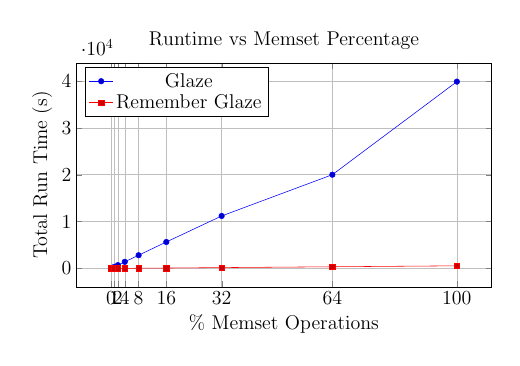
\begin{tikzpicture}[scale=0.5]
\begin{axis}[
    xlabel={\% Memset Operations},
    ylabel={Total Run Time (s)},
    title={Runtime vs Memset Percentage},
    xtick=data,
    xticklabels={0, 1, 2, 4, 8, 16, 32, 64, 100},
    grid=both,
    width=\textwidth,
    height=0.6\textwidth,
    ymajorgrids=true,
    xmajorgrids=true,
    legend style={at={(0.02,0.98)}, anchor=north west, font=\Large},
    label style={font=\Large},
    tick label style={font=\Large},
    title style={font=\Large}
]

% glaze_with_memset
\addplot coordinates {
    (0, 15.233870899)
    (1, 367.106329923)
    (2, 720.411448500)
    (4, 1423.994236935)
    (8, 2834.250849582)
    (16, 5652.903218061)
    (32, 11202.80643612)
    (64, 20000.132425532)
    (100, 39840.329482492)
};
\addlegendentry{Glaze}

% state_management_multi
\addplot coordinates {
    (0, 12.609255735)
    (1, 14.867499495)
    (2, 20.866470965)
    (4, 32.656366276)
    (8, 55.259813772)
    (16, 101.963029092)
    (32, 192.627531)
    (64, 371.358958)
    (100, 570.858858)
};
\addlegendentry{Remember Glaze}

\end{axis}
\end{tikzpicture}
\caption{Runtime comparison for \texttt{Glaze} (red) and \texttt{Remember glaze} (blue) as the percentage of \texttt{memset} function call transactions increases.}
\label{fig:memset}
\end{figure}

\subsubsection{Observations}
From Figure \ref{fig:memset}, a conspicuous divergence between \textit{Glaze} and \textit{Remember Glaze} emerges as the proportion of bulk write transactions increases. Initially, at 0\% bulk writes, both systems exhibit comparable performance, with \textit{Remember Glaze} slightly outperforming \textit{Glaze}. However, even a small increment in bulk writes drastically impacts \textit{Glaze}, as observed at merely 1\% bulk operations—execution time jumps from approximately 15 seconds to over 360 seconds. This exponential growth pattern continues as the bulk write percentage rises, reaching over 11,000 seconds at 32\%, and nearly 40,000 seconds at 100\% bulk operations.

In stark contrast, \textit{Remember Glaze} demonstrates remarkable resilience to increased bulk write percentages. Its runtime remains comparatively low and scales linearly rather than exponentially. Even at 100\% bulk writes, \textit{Remember Glaze}'s total execution time remains approximately 570 seconds—around 70 times faster than \textit{Glaze} under identical conditions. This demonstrates a clear performance advantage in handling large non-interdependent writes.

\subsubsection{Deductions}
The results conclusively validate the primary motivation behind \textit{Remember Glaze}. The exponential performance degradation observed in \textit{Glaze} highlights its inherent inefficiency in managing bulk writes. This inefficiency arises from \textit{Glaze}'s design, which mandates reading and rewriting entire chunks for each bulk write, severely amplifying I/O overhead and latency as bulk operations increase.

In contrast, \textit{Remember Glaze} employs a function-centric commit mechanism, treating bulk writes as atomic, constant-time operations. This design effectively eliminates the compounding I/O overhead characteristic of the original \textit{Glaze}, confirming that handling wide, non-interdependent writes as first-class operations is essential for maintaining high performance and stable latency.

Nevertheless, an underlying constraint remains pertinent—bulk write functions must exhibit spatial locality within individual chunks to leverage fully the benefits of \textit{Remember Glaze}'s design. Operations that span multiple chunks or lack spatial locality could still incur additional overhead due to increased cross-chunk dependencies during recovery. Therefore, careful tuning of chunk sizes and strategic spatial allocation of interdependent functions are critical considerations in practical deployments.

\subsection{Experiment 2: How does \textit{Remember Glaze} compare to \textit{WAL-snapshot}?}

\subsubsection{Introduction}
While Experiment 1 isolated the benefits of \textit{Remember Glaze} for bulk
updates, real deployments must also decide whether it is worth replacing the
well-understood \textit{WAL–snapshot} paradigm that still dominates mainstream
databases.  Experiment 2 therefore answers the core systems question:
\emph{How do the two approaches behave as the application state grows from a
few million to one hundred million accounts?}

\paragraph{Hypothesis.}
Because every \textit{WAL–snapshot} commit eventually triggers a
state-proportional checkpoint, we expect its throughput and latency to degrade
close to linearly with state size.  By contrast, \textit{Remember Glaze} writes
one fixed-size chunk per batch, so its steady-state cost should stay almost
constant; the price paid will surface in crash recovery, which must replay
more individual chunks as the state expands.

\paragraph{Methodology.}
Both engines are fed an identical synthetic workload of
\(50\,000\) batches (\(2^{16}\) transactions per batch, 95 \% transfers and
5 \% 64 KB range updates).  
Key parameters are held constant to ensure a fair comparison:

\begin{itemize}
  \item \textbf{Chunk size} in \textit{Remember Glaze}: 512 KB
        (shown in Experiment 3 to sit near the throughput sweet spot).
  \item \textbf{Snapshot interval} in the \textit{WAL–snapshot} setup:
        every \(1\,000\) batches, matching common production practice.
\end{itemize}

State size is scaled across six points—
\(2\), \(5\), \(10\), \(20\), \(50\), and
\(100\times10^{6}\) accounts—to expose any non-linearities.

\paragraph{Metrics captured.}
\vspace{-0.2em}
\begin{enumerate}
  \item \emph{Total execution time} for all \(50\,000\) batches, reflecting
        aggregate throughput (Fig.~\ref{fig:WAL_exec}).
  \item \emph{Median per-batch latency}, highlighting steady-state pause
        behaviour (Fig.~\ref{fig:WAL_per_batch}).
  \item \emph{Full-crash recovery time}, measured from process start to the
        first successful post-recovery commit
        (Fig.~\ref{fig:recovery_WAL}).
\end{enumerate}

Repeating each configuration five times and reporting the mean eliminates
noise from the host hypervisor and SSD wear-levelling.  The resulting data
provide a head-to-head picture of the scalability limits and operational
trade-offs of both persistence schemes.

\subsubsection{Results}

The experimental results are presented in Figures \ref{fig:WAL_exec}, \ref{fig:WAL_per_batch} and \ref{fig:recovery_WAL} showing the total execution time, per-batch runtime and recovery runtime as a function of the number of account.
\begin{figure}[H] 
\centering
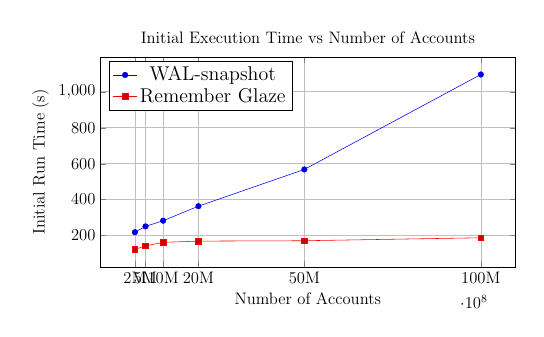
\begin{tikzpicture}[scale=0.5]
\begin{axis}[
    xlabel={Number of Accounts},
    ylabel={Initial Run Time (s)},
    title={Initial Execution Time vs Number of Accounts},
    xtick=data,
    xticklabels={2M, 5M, 10M, 20M, 50M, 100M},
    grid=both,
    width=\textwidth,
    height=0.57\textwidth,
    ymajorgrids=true,
    xmajorgrids=true,
    legend style={at={(0.02,0.98)}, anchor=north west, font=\Large},
    label style={font=\large},
    tick label style={font=\large},
    title style={font=\large}
]

\addplot coordinates {
    (2000000, 218.6284068)
    (5000000, 250.9743689)
    (10000000, 282.5195501)
    (20000000, 363.3880152)
    (50000000, 567.8183882)
    (100000000, 1096.113067)
};
\addlegendentry{WAL-snapshot}

\addplot coordinates {
    (2000000, 123.095114)
    (5000000, 142.8687522)
    (10000000, 162.0496913)
    (20000000, 169.0807597)
    (50000000, 171.1295201)
    (100000000, 187.641511)
};
\addlegendentry{Remember Glaze}

\end{axis}
\end{tikzpicture}
\caption{ WAL-snapshot's runtime in blue, \textit{Remember Glaze}'s in red as the size of the state increases.}
\label{fig:WAL_exec}
\end{figure}

\begin{figure}[H]   
\centering
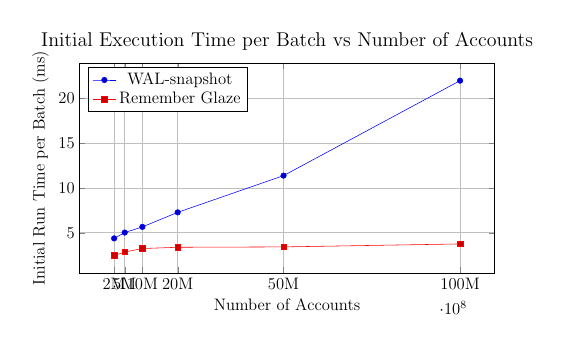
\begin{tikzpicture}[scale=0.5]
\begin{axis}[
    xlabel={Number of Accounts},
    ylabel={Initial Run Time per Batch (ms)},
    title={Initial Execution Time per Batch vs Number of Accounts},
    xtick=data,
    xticklabels={2M, 5M, 10M, 20M, 50M, 100M},
    grid=both,
    width=\textwidth,
    height=0.57\textwidth,
    ymajorgrids=true,
    xmajorgrids=true,
    legend style={at={(0.02,0.98)}, anchor=north west, font=\large},
    label style={font=\large},
    tick label style={font=\large},
    title style={font=\Large}
]

\addplot coordinates {
    (2000000, 4.372568)
    (5000000, 5.019487)
    (10000000, 5.650391)
    (20000000, 7.267760)
    (50000000, 11.356368)
    (100000000, 21.922261)
};
\addlegendentry{WAL-snapshot}

\addplot coordinates {
    (2000000, 2.461902)
    (5000000, 2.857375)
    (10000000, 3.240994)
    (20000000, 3.381615)
    (50000000, 3.422590)
    (100000000, 3.752830)
};
\addlegendentry{Remember Glaze}

\end{axis}
\end{tikzpicture}
\caption{\textit{WAL-snapshot} and \textit{Remember Glaze}’s runtimes as the number of elements in our state increases.}
\label{fig:WAL_per_batch}
\end{figure}
\begin{figure}[H]
\centering
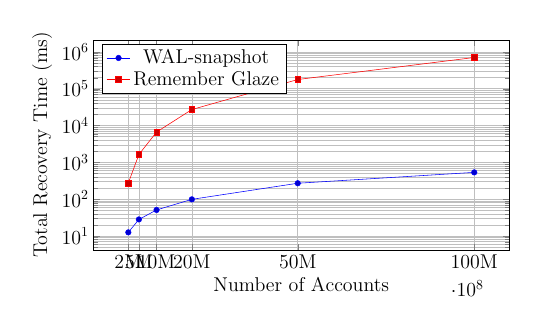
\begin{tikzpicture} [scale=0.5]
\begin{axis}[
    ylabel={Total Recovery Time (ms)},
    xlabel={Number of Accounts},
    legend style={at={(0.98,0.02)}, anchor=south east},
    ymode=log,
    xtick=data,
    xticklabels={2M, 5M, 10M, 20M, 50M, 100M},
    grid=both,
    width=\textwidth,
    height=0.57\textwidth,
    ymajorgrids=true,
    xmajorgrids=true,
    legend style={at={(0.02,0.98)}, anchor=north west, font=\Large},
    label style={font=\Large},
    tick label style={font=\Large},
    title style={font=\Large}
]
\addplot coordinates {
    (2000000, 12.518)
    (5000000,28.116)
    (10000000,50.878)
    (20000000,98.823)
    (50000000, 270.486)
    (100000000,534.065)
};
\addlegendentry{WAL-snapshot}
\addplot coordinates {
    (2000000,274.224)
    (5000000, 1633.504)
    (10000000, 6657.644 )
    (20000000, 27227.789)
    (50000000, 178141.801)
    (100000000, 707138.273)
};
\addlegendentry{Remember Glaze}
\end{axis}
\end{tikzpicture}
\caption{Comparing Remember glaze's and WAL-snapshot's recovery algorithms}
\label{fig:recovery_WAL}
\end{figure}

\subsubsection{Observations}

The performance metrics clearly illustrate significant differences between the two approaches. As state size grows, the total execution time of \textit{WAL-snapshot} increases substantially faster than \textit{Remember Glaze}. At 100 million accounts, \textit{WAL-snapshot} takes over five times longer than at 2 million accounts, highlighting its linear scalability constraint and considerable overhead due to snapshotting operations. In contrast, \textit{Remember Glaze}'s total execution time demonstrates only moderate growth, maintaining relatively stable per-batch latencies, irrespective of state size.

Further analysis of per-batch execution times confirms that \textit{Remember Glaze} maintains consistently low latencies, showing only minor increases as the number of accounts expands significantly. Conversely, \textit{WAL-snapshot} shows an increasingly steep rise in per-batch latency, indicating a marked performance degradation under large-scale workloads.

The third graph further illuminates the performance characteristics, specifically highlighting the recovery phase. \textit{WAL-snapshot} demonstrates a markedly superior recovery performance with recovery times growing relatively modestly, even at substantial account counts. In stark contrast, \textit{Remember Glaze} experiences exponential growth in recovery time as the number of accounts increases. At 100 million accounts, the recovery time for \textit{Remember Glaze} is dramatically higher compared to \textit{WAL-snapshot}, underscoring a key limitation of the architecture.

\subsubsection{Deductions}

These results validate the architectural advantages of \textit{Remember Glaze}. Specifically, its ability to perform constant-time, fixed-size writes per batch, irrespective of total state size, substantially reduces latency spikes inherent in \textit{WAL-snapshot} architectures.

The \textit{WAL-snapshot} method's need for periodic full state snapshots imposes a weighty performance penalty, especially notable in large-scale environments. This limitation can cause detrimental effects on high-throughput, latency-sensitive workloads, emphasizing the suitability of \textit{Remember Glaze} for modern applications requiring predictable, low-latency persistence.

However, a trade-off remains evident in the recovery phase. While \textit{Remember Glaze} achieves superior runtime performance under steady-state conditions, its recovery complexity grows rapidly with increasing state size due to the need to reconstruct the state from multiple small chunks. The third graph explicitly demonstrates this exponential growth in recovery time, highlighting the critical importance of optimizing recovery mechanisms. Consequently, tuning parameters such as chunk size become essential to balancing regular performance against recovery efficiency. Additionally, exploring approaches like rolling super-chunks or background checksum computations could considerably alleviate the identified bottleneck in recovery performance.


\subsection{Experiment 3: What effects do the chunk sizes have \textit{Remember Glaze}'s performance in recovery and transaction processing?}
\subsubsection{Introduction}
Chunk size is the single most powerful “dial’’ exposed by \textit{Remember Glaze}:  
it determines (i) how much data must be written to the checkpoint ring on every
commit and (ii) how many distinct snapshots and log fragments have to be scanned
during crash recovery.  Experiment 3 therefore investigates \emph{how varying the
chunk size influences both steady-state throughput and recovery latency}.  

\paragraph{Hypothesis.}
Increasing the chunk size should shorten recovery—because fewer, larger chunks
have to be loaded and replayed—but at the cost of higher per-batch I/O, which
will in turn inflate processing time and median batch latency.  We expect to
observe a clear trade-off curve with a “sweet spot’’ that balances the two
opposing effects.

\paragraph{Methodology.}
We fix all other parameters and vary the chunk size across seven powers of two
(256;512;1024;2048;4096;8192;16384) KB.  For each chunk size we
run an identical synthetic workload of \(50{,}000\) batches, each batch
containing \(2^{16}\) transactions (95 \% random pairwise transfers, 5 \%
\texttt{memset}-style range updates).  The experiment is repeated for four state
sizes—\(1\), \(10\), \(50\), and \(100\times10^{6}\) accounts—to assess how the
trade-off shifts with scale.  Every configuration is executed five times on the
same \texttt{c7gd.8xlarge} instance; we report the mean values.

\paragraph{Metrics recorded.}
\begin{itemize}
  \item \textbf{Recovery time for each run} (Fig.~\ref{fig:chunk_size_effect}): time to
        restore the full state and reach the first post-crash commit.
  \item \textbf{Total processing time} over all \(50{,}000\) batches
        (Fig.~\ref{fig:chunk_size_processingtime}).
  \item \textbf{Median per-batch latency} measured at the 50th percentile
        (Fig.~\ref{fig:chunk_per_batch}), which filters out occasional GC or
        OS-level noise and highlights the systematic cost of larger snapshots.
\end{itemize}

This controlled sweep isolates the impact of chunk size and provides concrete
guidance for operators looking to tune \textit{Remember Glaze} to a given
throughput target or recovery-time objective.
\subsubsection{Results}
The results for this experiment are in figures \ref{fig:chunk_size_effect} through \ref{fig:chunk_size_processingtime} and show the effects of chunk sizes on state recovery speed as well as general processing performance.

\FloatBarrier
\begin{figure}[H]  
\centering
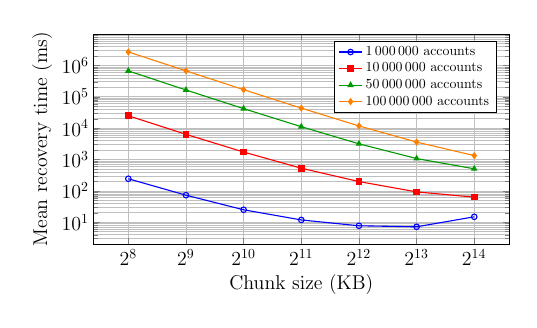
\begin{tikzpicture} [scale=0.5]
  \begin{axis}[
    xlabel={Chunk size (KB)},
    ylabel={Mean recovery time (ms)},
    xmode=log,
    log basis x=2,
    ymode=log,
    log basis y=10,
    width=\textwidth,
    height=0.57\textwidth,
    grid=both,
    legend pos=north east,         
    legend cell align=left,
    label style={font=\Large},
    tick label style={font=\Large},
    title style={font=\Large}
  ]
    % 1,000,000 accounts (blue)
    \addplot[
      color=blue,
      thick,
      mark=o
    ] coordinates {
      (256,242.36) (512,72.58) (1024,24.83) (2048,11.79)
      (4096,7.67)  (8192,7.12)  (16384,14.84)
    };
    \addlegendentry{1\,000\,000 accounts}

    % 10,000,000 accounts (red)
    \addplot[
      color=red,
      thick,
      mark=square*
    ] coordinates {
      (256,24761.70) (512,6325.51) (1024,1723.51) (2048,526.02)
      (4096,197.12)  (8192,92.50)   (16384,62.74)
    };
    \addlegendentry{10\,000\,000 accounts}

    % 50,000,000 accounts (green)
    \addplot[
      color=green!60!black,
      thick,
      mark=triangle*
    ] coordinates {
      (256,668003.31) (512,164187.71) (1024,41697.83) (2048,11082.34)
      (4096,3156.18)  (8192,1067.92)   (16384,503.17)
    };
    \addlegendentry{50\,000\,000 accounts}

    % 100,000,000 accounts (orange)
    \addplot[
      color=orange,
      thick,
      mark=diamond*
    ] coordinates {
      (256,2683589.56) (512,671010.94) (1024,167891.80) (2048,43236.38)
      (4096,11711.41)  (8192,3580.31)   (16384,1330.05)
    };
    \addlegendentry{100\,000\,000 accounts}

  \end{axis}
\end{tikzpicture}
\caption{Recovery time as the size of the chunks increases.}
\label{fig:chunk_size_effect}
\end{figure}

\begin{figure}[H]  
\centering
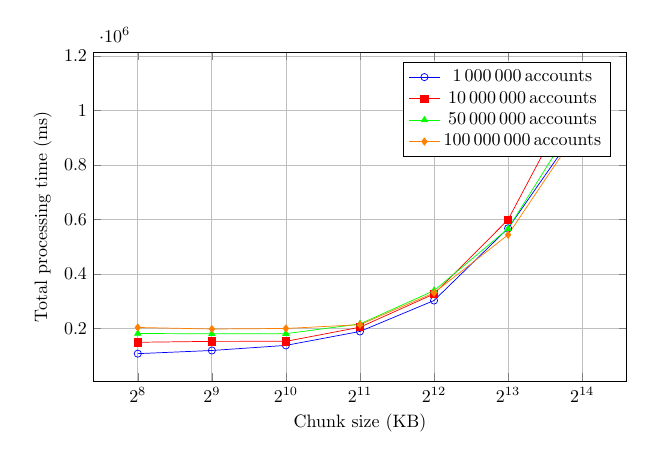
\begin{tikzpicture}[scale=0.65]
  \begin{axis}[
    xlabel={Chunk size (KB)},
    ylabel={Total processing time (ms)},
    xmode=log,
    log basis x={2},
    xtick={256,512,1024,2048,4096,8192,16384},
    legend entries={
      {1\,000\,000\,accounts},
      {10\,000\,000\,accounts},
      {50\,000\,000\,accounts},
      {100\,000\,000\,accounts}
    },
    legend pos=north east,
    grid=both,
    width=12cm,
    height=8cm,
  ]

    %--- 1,000,000 accounts ---
    \addplot[color=blue, mark=o] coordinates {
      (256,107992.1)
      (512,119583.6)
      (1024,138306.1)
      (2048,189436.3)
      (4096,302998.9)
      (8192,568206.5)
      (16384,957277.8)
    };

    %--- 10,000,000 accounts ---
    \addplot[color=red, mark=square*] coordinates {
      (256,149713.2)
      (512,153077.3)
      (1024,153146.4)
      (2048,205017.8)
      (4096,327150.2)
      (8192,599881.6)
      (16384,1112721.5)
    };

    %--- 50,000,000 accounts ---
    \addplot[color=green, mark=triangle*] coordinates {
      (256,181870.0)
      (512,180977.8)
      (1024,181414.0)
      (2048,217083.9)
      (4096,339234.8)
      (8192,566648.9)
      (16384,1002220.2)
    };

    %--- 100,000,000 accounts ---
    \addplot[color=orange, mark=diamond*] coordinates {
      (256,204081.6)
      (512,198435.7)
      (1024,200459.0)
      (2048,214279.6)
      (4096,331305.9)
      (8192,544342.4)
      (16384,948534.2)
    };

  \end{axis}
\end{tikzpicture}
\caption{Processing time as the size of the chunks increases.}
\label{fig:chunk_size_processingtime}
\end{figure}

\begin{figure}[H]
\centering    
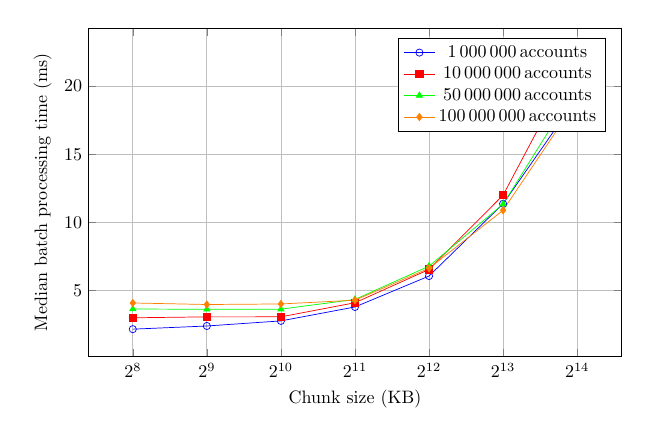
\begin{tikzpicture}[scale=0.65]
  \begin{axis}[
    xlabel={Chunk size (KB)},
    ylabel={Median batch processing time (ms)},
    xmode=log,
    log basis x={2},
    xtick={256,512,1024,2048,4096,8192,16384},
    legend entries={
      {1\,000\,000\,accounts},
      {10\,000\,000\,accounts},
      {50\,000\,000\,accounts},
      {100\,000\,000\,accounts}
    },
    legend pos=north east,
    grid=both,
    width=12cm,
    height=8cm,
  ]

    %--- 1,000,000 accounts ---
    \addplot[color=blue, mark=o] coordinates {
      (256,  2.159841)
      (512,  2.391671)
      (1024, 2.766122)
      (2048, 3.788726)
      (4096, 6.059978)
      (8192,11.364129)
      (16384,19.145556)
    };

    %--- 10,000,000 accounts ---
    \addplot[color=red, mark=square*] coordinates {
      (256,  2.994264)
      (512,  3.061546)
      (1024, 3.062927)
      (2048, 4.100355)
      (4096, 6.543005)
      (8192,11.997632)
      (16384,22.254429)
    };

    %--- 50,000,000 accounts ---
    \addplot[color=green, mark=triangle*] coordinates {
      (256,  3.637400)
      (512,  3.619556)
      (1024, 3.628281)
      (2048, 4.341679)
      (4096, 6.784697)
      (8192,11.332979)
      (16384,20.044404)
    };

    %--- 100,000,000 accounts ---
    \addplot[color=orange, mark=diamond*] coordinates {
      (256,  4.081631)
      (512,  3.968713)
      (1024, 4.009179)
      (2048, 4.285592)
      (4096, 6.626119)
      (8192,10.886848)
      (16384,18.970684)
    };

  \end{axis}
\end{tikzpicture}
\caption{Median per-batch latency versus chunk size}
\label{fig:chunk_per_batch}
\end{figure}
\FloatBarrier
\subsubsection{Observations}
Figures~\ref{fig:chunk_size_effect}–\ref{fig:chunk_per_batch} reveal a clear, antagonistic relationship between chunk size and the two main performance axes of \textit{Remember Glaze}:

\begin{enumerate}
  \item \textbf{Recovery performance improves super-linearly with larger chunks.}
        For every workload size the mean recovery time drops by almost two
        orders of magnitude when moving from 256 KB to
        4 MB chunks, and continues to fall—albeit more gently—up to
        8.  Beyond that point the curve flattens (and even
        rebounds slightly for the smallest dataset). This is because of the fact that at that point 16 MB is greater than the size of the state.
  \item \textbf{Steady-state throughput deteriorates roughly linearly with
        chunk size.}
        The total runtime in Fig.~\ref{fig:chunk_size_processingtime} stays
        almost flat up to 1 MB, then rises sharply; at
        16 MB chunks the end-to-end job completes \(\approx7{-}9\times\)
        slower than with 256 KB chunks. The same trend appears
        in the median per-batch latency (Fig.~\ref{fig:chunk_per_batch}), which climbs from {\(\sim\)2–4 ms} at sub-MB chunks to {\(\sim\)18–22 ms} at 16 MB.
  \item \textbf{The “knee” of the curve shifts with state size.}
        Larger datasets profit longer from increasing the chunk size: for
        \(100\times10^{6}\) accounts the recovery curve keeps falling up to
        16 MB, whereas for \(1\times10^{6}\) accounts the optimal
        point is already reached around 8 MB.  In contrast, batch
        latency begins to climb after 1 MB almost
        independently of dataset size.
\end{enumerate}

\subsubsection{Deductions}
The data confirm the intuitive trade-off built into the design:

\begin{itemize}
  \item \emph{Why recovery accelerates with larger chunks.}  
        Fewer, bigger chunks translate to fewer random seeks and fewer replay
        passes during crash recovery.  Because the recovery algorithm is
        \(O(N_{\text{chunks}})\) for snapshot loading and
        \(O(N_{\text{chunks}}\!\times\!B)\) for log replay, halving
        \(N_{\text{chunks}}\) roughly halves the amount of work in both phases,
        explaining the near-hyperbolic drop in Fig.~\ref{fig:chunk_size_effect}.
  \item \emph{Why processing slows down with larger chunks.}
        Every commit writes an entire chunk snapshot.  As the chunk grows, the
        amount of data copied from DRAM to the NVMe device (and checksummed)
        scales linearly; once the snapshot no longer fits in the LLC, memory
        bandwidth—not SSD throughput—becomes the bottleneck, producing the
        quasi-exponential wall in Figs.~\ref{fig:chunk_size_processingtime}
        and~\ref{fig:chunk_per_batch}.
  \item \emph{Choosing an operating point.}
        For small and medium deployments (up to \(\sim\!10^{7}\) accounts) a
        chunk size between 512 KB and 1 MB offers a
        sweet spot: recovery remains below one second while batch latency
        stays within the 3 ms envelope needed for
        high-throughput workloads.  
        At very large scales the pendulum swings: moving to
        4 MB \textendash 8 MB chunks reduces worst-case
        recovery from minutes to seconds at the cost of single-digit-millisecond
        extra latency per batch—often an acceptable trade-off for chains or
        ledgers that prioritise fast restart times.
  \item \emph{Implications for autotuning.}
        Because the optimal chunk size depends on both state size and
        recovery-time objective (RTO), a static compile-time constant is
        sub-optimal.  A promising avenue is \textbf{adaptive chunking}: the
        system could start with small chunks for low latency, then merge them
        into “super-chunks’’ in the background once the state crosses a
        configurable threshold or during periods of low traffic, thereby
        shortening future recoveries without impacting peak throughput.
\end{itemize}

In summary, Experiment 3 quantifies the fundamental dial exposed by
\textit{Remember Glaze}: tuning chunk size lets operators trade a linear
increase in steady-state latency for an inverse-exponential decrease in crash
recovery time.  Practical deployments should therefore pick the smallest chunk
that still meets their RTO, or implement an adaptive policy that converges on
that value automatically.

\subsection{Conclusion}
This evaluation demonstrates that \textit{Remember Glaze} effectively achieves its primary objectives: maintaining consistently high throughput and low latency for transaction processing, particularly under workloads involving frequent, large-scale bulk updates such as \texttt{memset}-type operations. Compared to the conventional WAL–snapshot architecture, \textit{Remember Glaze} significantly improves batch-processing performance, achieving a 40–70\% reduction in batch-execution times across all tested state sizes. Furthermore, it entirely eliminates the periodic latency spikes typically caused by the snapshotting of large data sets, thus ensuring smoother and more predictable performance.

Additionally, when benchmarked against the original \textit{glaze} algorithm, \textit{Remember Glaze} consistently sustains stable operation even under intense workloads that previously led to performance degradation. This highlights the effectiveness of the design choices made to specifically accommodate bulk-update operations.

Nevertheless, these performance enhancements introduce certain trade-offs. The chunk-based architecture, while advantageous during routine batch processing, results in increased complexity and time required for state recovery after crashes or system restarts. Specifically, the recovery duration scales proportionally with the number of chunks, which is directly influenced by both the overall state size and the chosen chunk dimensions. Consequently, recovery performance can degrade markedly for very large deployments involving tens or hundreds of millions of accounts, potentially exceeding the recovery times associated with the WAL–snapshot method.

An important implication is that the choice of chunk size becomes critical. Smaller chunks reduce the overhead of real-time persistence and improve regular transaction throughput, whereas larger chunks substantially speed up recovery procedures by minimizing the total chunk count. Selecting an optimal chunk size is therefore workload-specific and might require dynamic adjustments during different phases of system deployment.

In conclusion, \textit{Remember Glaze} represents a practical and effective compromise between standard snapshot-based systems and fully in-memory solutions. It is particularly suitable for applications demanding high performance in transaction processing with frequent bulk updates, such as modern blockchain systems or real-time analytics platforms. While recovery complexity presents a notable challenge, it is manageable through thoughtful system tuning and design trade-offs. Future improvements might explore adaptive chunk sizing, hybrid recovery mechanisms to improve recovery times, and enhanced support for functions spanning multiple chunks without compromising crash safety.


\section{Related Work}

Durability techniques in modern data stores fall into two broad families.  
\textbf{Write-ahead logging with periodic snapshots}, popularized by the ARIES
recovery algorithm \cite{mohan1992aries}, offers strong crash consistency but
incurs state-proportional latency spikes whenever a full checkpoint is flushed
to disk. Production systems such as PostgreSQL and Cassandra still expose this behavior once their datasets reach tens of gigabytes.

\textbf{Log-structured designs}—originating with the Log-Structured File
System \cite{rosenblum1992lfs} and later refined into Log-Structured
Merge-trees (LSM) \cite{ongaro2020efficient}—transform every update into a
sequential append, greatly improving steady-state throughput.  However, background
compaction and segment cleaning re-introduce stalls that grow with data volume.

Work on \textbf{incremental or chunk-based checkpointing} tries to break
this dependency by persisting only the delta since the last snapshot.  Apache Flink’s incremental checkpoints \cite{carbone2015flink} and Oracle’s buffer-pool increments \cite{kalantar1998oracle} shorten pause times but still require occasional full materialization.

\textbf{Remember Glaze} extends the chunked idea one step further: the system
never dumps the complete state.  Instead, it commits exactly one fixed-size
chunk per batch into a pre-allocated circular ring log.  This choice guarantees
constant-time commits, a deterministically bounded on-disk footprint, and
native support for bulk, non-interdependent operations—properties that, to our
knowledge, no prior scheme achieves simultaneously.

\section{Conclusion \& Future Development}

\subsubsection*{Future Work}
The evaluation presented in this project demonstrates that \textit{Remember Glaze} successfully meets its primary design goals, while also uncovering areas for further improvement and research. Here are a few ideas that could be explored:

\paragraph{Memory Bandwidth as the Next Bottleneck}
Beyond certain chunk sizes that exceed the last-level cache, the bottleneck shifts from SSD write speeds to DRAM bandwidth and checksum computation performance. Testing on the AWS \texttt{c7gd.8xlarge} instance revealed that memory copying and checksum computations saturate around 180GB/s, tellingly outpacing the SSD's maximum throughput of approximately 11GB/s. This indicates that improvements in storage speed alone will not boost overall throughput without first addressing memory bandwidth constraints, potentially through optimized data paths like non-temporal memory stores or SIMD instructions.

\paragraph{Checksum Validation Overhead}
Checksum validation, specifically full-chunk CRC32 checks, introduces a substantial overhead (8–15\%) at chunk sizes of \(4\text{–}8\,\text{MB}\). Future optimizations, such as offloading checksum computation to background threads or exploiting ARMv9 hardware CRC instructions, could significantly reduce this overhead without compromising fault detection reliability.
\(4\text{–}8\,\text{MB}\). 

\paragraph{Enhancing Recovery Performance}
Recovery performance degrades more quickly compared to traditional WAL-snapshot approaches for very large states. A promising solution identified in this project is the concept of \textit{rolling super-chunks}. Periodically saving an XOR-folded auxiliary snapshot of \(k\) contiguous chunks can reduce the required replay passes from \(N\) to \(N/k\), incurring only \(1/k\) additional write amplification cost.

\subsubsection*{Conclusion}
This bachelor project aimed to reconcile three traditionally conflicting objectives within persistent storage systems: \emph{high throughput}, \emph{predictable latency}, and \emph{robust crash-safety}. The developed solution, \textit{Remember Glaze}, successfully integrates these goals using a chunk-oriented checkpoint ring log architecture. This design limits synchronous I/O operations to fixed-size regions, delivering predictable performance and enhanced durability.

\paragraph{Main Findings}
\begin{itemize}
\item Strict separation between in-memory computation and asynchronous durability ensures constant-time batch commits, unaffected by the overall state size.
\item Testing on AWS \texttt{c7gd.8xlarge} demonstrated that \textit{Remember Glaze} reduces batch latency by 40–70% compared to WAL-snapshot, eliminating snapshot-induced interruptions.
\item Disk space utilization remains predictably bounded, effectively addressing the unlimited growth typical of traditional write-ahead logging systems.
\end{itemize}

\paragraph{Limitations}
Recovery times scale significantly with an increasing number of chunks, and operations spanning multiple chunks must adhere to strict spatial-locality constraints.

\paragraph{Summary}
\textit{Remember Glaze} illustrates that careful selection of chunk granularity combined with a structured circular log can deliver robust performance and reliability with moderate implementation complexity. The principles and results presented here establish a solid basis for future developments in high-performance persistent data storage systems.

\begin{thebibliography}{9}

\bibitem{mohan1992aries}
C.~Mohan, D.~Haderle, B.~Lindsay, H.~Pirahesh, and P.~Schwarz.
\newblock ARIES: A transaction recovery method supporting fine‐granularity
  locking and partial rollbacks using write‐ahead logging.
\newblock \emph{ACM Transactions on Database Systems}, 17(1):94–162, 1992.

\bibitem{rosenblum1992lfs}
M.~Rosenblum and J.~K. Ousterhout.
\newblock The design and implementation of a log‐structured file system.
\newblock \emph{ACM Transactions on Computer Systems}, 10(1):26–52, 1992.

\bibitem{ono1996lsm}
P.~O’Neil, E.~Cheng, D.~Gawlick, and E.~O’Neil.
\newblock The log‐structured merge‐tree (LSM‐Tree).
\newblock \emph{Acta Informatica}, 33(4):351–385, June 1996.

\bibitem{carbone2015flink}
P.~Carbone, S.~Ewen, G.~Fóra, S.~Haridi, and K.~Tzoumas.
\newblock Lightweight asynchronous snapshots for distributed dataflows.
\newblock In \emph{Proceedings of the 2015 Symposium on Cloud Computing (SoCC)}, pages 421–435. ACM, 2015.

\bibitem{kalantar1998oracle}
Oracle Corporation.
\newblock Checkpointing in Oracle 8.0.
\newblock In \emph{Proceedings of the 24th VLDB Conference}, pages 665–676. ACM, 1998.

\end{thebibliography}
\end{document}
